\chapter{Standalone Bundles: \texttt{guix pack} for Docker, AppImage, and HPC}
\label{chap:guix-pack}

\epigraph{``The true test of a reproducible deployment is not whether it runs on your machine, but whether it runs on an ancient Red Hat 7 cluster managed by sysadmins who forbid root access, disable internet connectivity, and refuse to install Guix.''}{--- The HPC Vagabond}

\noindent
Up to this point in our journey, we have enjoyed the paradise of having GNU Guix installed on our systems. Whether managing user profiles, spawning disposable \guixcmd{guix shell} containers, or declaring our entire workstation via Guix System, the \texttt{guix-daemon} and the immutable store (\texttt{/gnu/store}) were always there to orchestrate reality.

\begin{tearsbox}[The Real-World Transfer Dilemma]
What happens when you need to deploy your software to:
\begin{itemize}
  \item A corporate cloud Kubernetes cluster where nodes only accept Docker or OCI container images?
  \item A massive institutional High-Performance Computing (HPC) supercomputer with thousands of nodes running CentOS 7 or RHEL 8, where sysadmins strictly forbid root access, block outbound internet access, and refuse to install GNU Guix?
  \item A colleague's vanilla Ubuntu or Fedora laptop where they just want a single, zero-dependency executable they can double-click or run from the terminal without installing Guix?
\end{itemize}
\end{tearsbox}

Traditional answers to this problem are depressing: you either write a 60-line, non-reproducible \texttt{Dockerfile} that pulls mutable APT mirrors and \texttt{pip} wheels, or you spend days fighting dynamic linker errors (\texttt{version `GLIBC\_2.34' not found}) trying to build static binaries.

GNU Guix offers a revolutionary escape hatch: \guixcmd{guix pack}.

\section{The Philosophy of \texttt{guix pack}}

In Guix, every package in \texttt{/gnu/store} is already a self-contained, immutable artifact whose complete dependency graph is known to the byte. 

Because Guix calculates the exact \textbf{closure} (the target package plus every single shared library, interpreter, data file, configuration script, and runtime dependency it requires), Guix can extract that sub-graph from \texttt{/gnu/store} and pack it into whatever standalone format the outside world demands:

\begin{enumerate}
  \item \textbf{Standalone Tarballs (\texttt{-f tar})}: Unpack anywhere, with optional execution wrappers.
  \item \textbf{Docker / OCI Images (\texttt{-f docker})}: Layered, bit-for-bit reproducible container images with zero base-OS bloat.
  \item \textbf{AppImage Bundles (\texttt{-f appimage})}: Single-file executables with embedded squashfs runtimes for any Linux desktop.
  \item \textbf{Debian / RPM Packages (\texttt{-f deb}, \texttt{-f rpm})}: Standard system packages containing the relocatable Guix closure for legacy server fleets.
  \item \textbf{SquashFS Images (\texttt{-f squashfs})}: Read-only compressed images ideal for Singularity, Apptainer, and HPC network filesystems.
\end{enumerate}

Crucially, \textbf{Guix does not need Docker to build Docker images}, nor does it need AppImage toolkits or Debian build tools. It creates all of these archives directly from the store graph with bit-for-bit reproducibility.

\section{The Relocatability Miracle: How Non-Guix Systems Run Store Binaries}

There is an obvious technical hurdle: binaries compiled by Guix have their runtime library paths (\texttt{RUNPATH}) hardcoded to absolute paths inside \texttt{/gnu/store/...}. 

If you copy these binaries to a machine that does not have \texttt{/gnu/store} mounted, any attempt to launch them fails immediately with:
\begin{center}
\texttt{bash: ./bin/python3: No such file or directory}
\end{center}
The Linux dynamic linker (\texttt{ld-linux.so}) cannot find its interpreter at \texttt{/gnu/store/...}!

How does \guixcmd{guix pack} solve this without requiring root access on the target machine? It provides three distinct \textbf{relocation wrappers} via the \texttt{-R} (or \texttt{--relocatable}) flag:

\subsection{1. User Namespaces (The Default)}
On modern Linux kernels (version 3.10+), an unprivileged user can create a mount namespace (using the \texttt{clone(2)} or \texttt{unshare(2)} system calls). 
When you invoke a relocatable binary produced with \texttt{guix pack -R}, a lightweight C launcher executes first. It creates an unprivileged user and mount namespace, mounts the unpacked directory onto a virtual \texttt{/gnu/store} visible only to that process tree, and executes the target program. To the application, \texttt{/gnu/store} exists perfectly, while the host filesystem remains untouched!

\subsection{2. PRoot Fallback}
Some hardened institutional clusters or older Linux kernels disable unprivileged user namespaces (\texttt{kernel.unprivileged\_userns\_clone = 0}). In this scenario, the wrapper automatically falls back to **PRoot** (which intercepts filesystem system calls via \texttt{ptrace(2)} to translate \texttt{/gnu/store} accesses transparently in user space).

\subsection{3. Fakechroot Fallback}
As a final lightweight fallback, Guix can employ an \texttt{LD\_PRELOAD} wrapper that intercepts standard C library file functions.

\begin{alchemybox}[The Execution Ladder]
By passing \guixcmd{--relocatable} (or \guixcmd{-R}), Guix generates binaries that try:
\begin{center}
\textbf{User Namespaces} $\longrightarrow$ (fallback) $\longrightarrow$ \textbf{PRoot}
\end{center}
Your package will run on virtually \textbf{any} Linux machine from the past 15 years, unprivileged, without installing Guix or Docker!
\end{alchemybox}

\section{Packaging for High-Performance Computing (HPC)}

HPC clusters represent the most common battleground for relocatable bundles. Imagine you have built a complex computational pipeline using Python, NumPy, SciPy, and OpenMPI. The target cluster runs Red Hat Enterprise Linux 7 with no internet access and no Guix.

\subsection{Building a Self-Contained Tarball}

Let us package Python and your analysis tools into a standalone, relocatable tarball:

\begin{lstlisting}[style=guixcli]
# Generate a relocatable tarball with symlinks for convenient execution
guix pack -R \
  -S /bin=bin \
  -S /lib=lib \
  -S /share=share \
  python python-numpy python-scipy \
  -C xz
\end{lstlisting}

Let us dissect the flags:
\begin{itemize}
  \item \guixcmd{-R} (or \guixcmd{--relocatable}): Wraps all executables with the user-namespace / PRoot relocation launcher.
  \item \guixcmd{-S /bin=bin}: Creates a top-level \texttt{bin/} symlink pointing to the profile's \texttt{bin/} directory inside the archive. This ensures you can unpack and immediately run \texttt{./bin/python3}.
  \item \guixcmd{-C xz}: Compresses the output archive using XZ (options include \texttt{gzip}, \texttt{bzip2}, \texttt{zstd}, \texttt{none}).
\end{itemize}

Guix builds the closure, assembles the archive, and prints the path of the generated tarball:
\begin{center}
\texttt{/gnu/store/3x9k1p...-tarball-pack.tar.xz}
\end{center}

\subsection{Deploying and Running on the HPC Cluster}

Now, transfer this tarball to the remote supercomputer using \texttt{scp} or an external drive:

\begin{lstlisting}[style=guixcli]
# On your local Guix workstation:
scp /gnu/store/3x9k1p...-tarball-pack.tar.xz user@cluster.hpc.edu:~/

# On the remote supercomputer (which has NO Guix installed):
ssh user@cluster.hpc.edu
mkdir -p ~/my-env && cd ~/my-env
tar -xf ~/3x9k1p...-tarball-pack.tar.xz

# Execute immediately without root permissions!
./bin/python3 -c "import numpy, scipy; print('HPC Success with NumPy', numpy.__version__)"
\end{lstlisting}

Notice what just happened: the cluster node has no \texttt{/gnu/store}, no internet access, and ancient system libraries. Yet Python, NumPy, OpenBLAS, and GCC runtime libraries executed flawlessly in user space!

\subsection{Submitting SLURM Batch Jobs}

You can directly submit your relocatable bundle in SLURM or PBS/Torque batch submission scripts:

\begin{lstlisting}[style=guixcli]
#!/bin/bash
#SBATCH --job-name=guix_sim
#SBATCH --nodes=4
#SBATCH --ntasks-per-node=16
#SBATCH --time=12:00:00

# Execute simulation using our unpacked relocatable Guix environment
~/my-env/bin/python3 ~/scripts/distributed_simulation.py --input /data/raw.h5
\end{lstlisting}

\section{Direct Store Transfers: \texttt{guix copy} and \texttt{guix archive}}

If the remote machine or cluster \emph{does} have GNU Guix installed (such as a cluster where sysadmins run the \texttt{guix-daemon}), you do not even need to pack tarballs. You can beam store items directly across SSH connections.

\subsection{Zero-Friction Transfer with \texttt{guix copy}}

\guixcmd{guix copy} transfers a package and its complete closure over an SSH pipe directly into the remote daemon's store:

\begin{lstlisting}[style=guixcli]
# Copy the entire closure of R and Bioconductor to the remote cluster
guix copy --to=user@cluster.hpc.edu r r-deseq2

# Or pull an environment built on a fast build farm down to your local laptop
guix copy --from=builder.internal.net /gnu/store/8j29...-large-model
\end{lstlisting}

Because Guix checks store hashes on both sides, it transfers **only the missing store items**! If the remote machine already has GLIBC and Python, \guixcmd{guix copy} only beams over the delta.

\subsection{Air-Gapped Transfers with \texttt{guix archive}}

For military, medical, or secure air-gapped systems that are physically disconnected from the internet and have no SSH access:

\begin{lstlisting}[style=guixcli]
# 1. Export package closure to an authenticated binary archive file
guix archive --export -r python python-pytorch > pytorch-closure.nar

# 2. Walk the USB drive across the air-gap to the secure facility

# 3. Import directly into the secure machine's Guix store
guix archive --import < pytorch-closure.nar
\end{lstlisting}

The archive is cryptographically signed with your private key and authenticated by the recipient machine's authorized keys.

\section{Docker and OCI Images Without Docker: \texttt{-f docker}}

Traditional \texttt{Dockerfile} workflows are an operational nightmare:
\begin{lstlisting}[style=guixcli]
# The Traditional Anti-Pattern: Fragile, non-reproducible, bloated
FROM ubuntu:22.04
RUN apt-get update && apt-get install -y python3 python3-pip curl gcc \
    && rm -rf /var/lib/apt/lists/*
RUN pip3 install torch torchvision --extra-index-url https://...
COPY . /app
CMD ["python3", "/app/server.py"]
\end{lstlisting}
This Dockerfile violates every tenet of engineering reliability:
\begin{itemize}
  \item \textbf{Non-reproducible}: Running this tomorrow pulls different Ubuntu security patches and different \texttt{pip} wheels.
  \item \textbf{Bloated}: You ship a package manager (\texttt{apt}), systemd stubs, man pages, documentation, and build caches you will never use in production.
  \item \textbf{Privileged Daemon}: Building requires the Docker daemon running with root privileges on the host.
\end{itemize}

\subsection{Building a Minimal Docker Image with \texttt{guix pack}}

With \guixcmd{guix pack}, Guix constructs the Docker image archive directly from its dependency graph without running Docker:

\begin{lstlisting}[style=guixcli]
# Generate an ultra-lean, reproducible Docker image
guix pack -f docker \
  -S /bin=bin \
  -S /lib=lib \
  --entry-point=bin/guile \
  guile
\end{lstlisting}

Let us examine a real-world web microservice example packaging Python, Uvicorn, and a REST API:

\begin{lstlisting}[style=guixcli]
guix pack -f docker \
  -S /bin=bin \
  -S /etc=etc \
  --entry-point=bin/uvicorn \
  python python-uvicorn python-fastapi nss-certs
\end{lstlisting}

\begin{figure}[htbp]
\centering
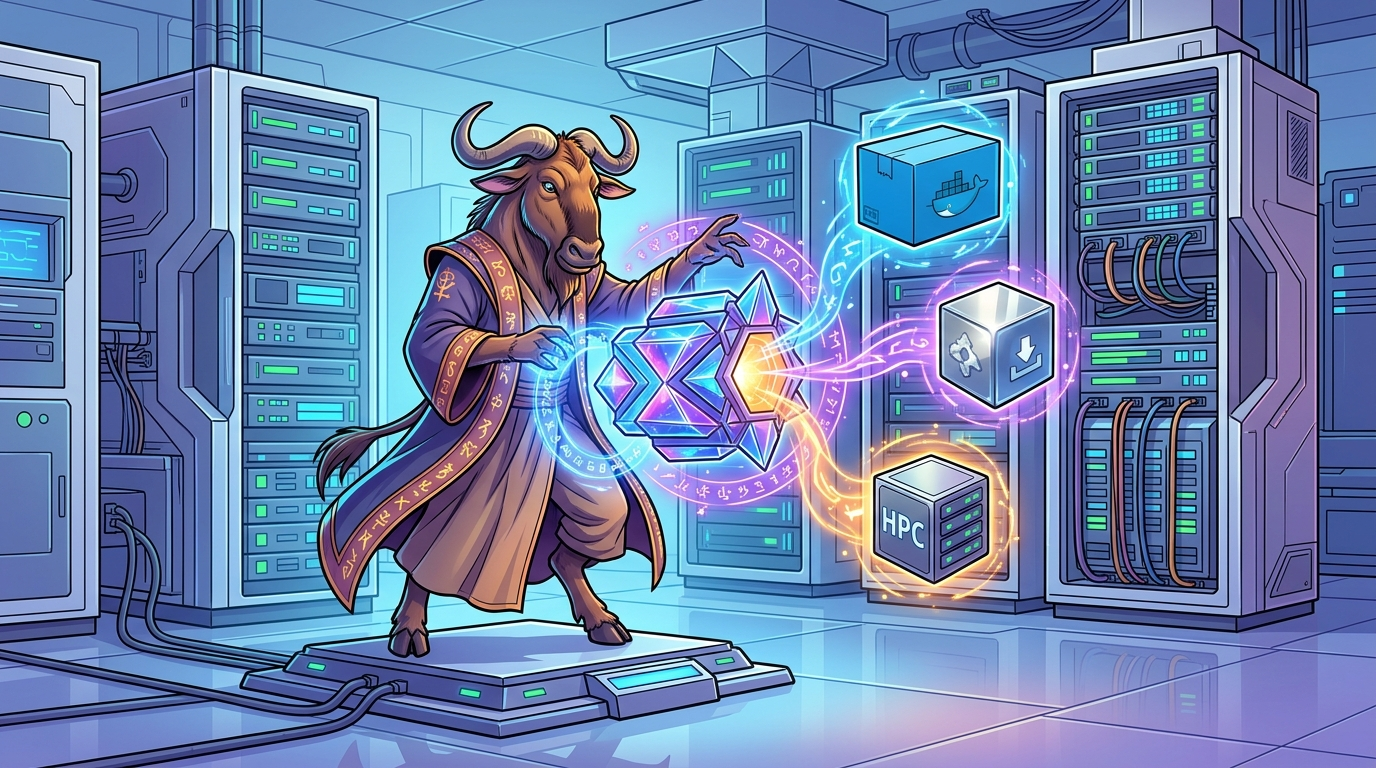
\includegraphics[width=0.92\textwidth]{images/guix_pack_diagram.jpg}
\caption*{\textit{Figure 12.1: From pure Scheme store graph to production: \guixcmd{guix pack} producing bit-for-bit identical Docker, AppImage, and HPC tarballs with zero host dependencies.}}
\end{figure}

\subsection{Loading and Running in Docker / Podman}

The resulting \texttt{.tar.gz} file is a valid OCI/Docker image. You can load and run it on any Kubernetes cluster, AWS ECS, or local Docker daemon:

\begin{lstlisting}[style=guixcli]
# Load image into Docker or Podman
docker load < /gnu/store/7q8m...-docker-pack.tar.gz

# Inspect image size and history
docker images
# REPOSITORY          TAG                 IMAGE ID            SIZE
# guile-fastapi       latest              4f8c9b2a1e0d        82.4MB

# Run the container
docker run -p 8000:8000 guile-fastapi:latest
\end{lstlisting}

\begin{alchemybox}[Why Guix Docker Images Are Superior]
\begin{enumerate}
  \item \textbf{Bit-for-Bit Reproducible}: Two developers compiling the same package commit with \guixcmd{guix pack -f docker} generate Docker images with the exact same SHA-256 image ID!
  \item \textbf{Attack Surface Reduction}: There is no \texttt{/bin/sh}, no package manager, no compiler, and no unnecessary binaries inside the container unless you explicitly declare them. If an attacker discovers an injection vulnerability, there are no shells or system utilities to exploit!
  \item \textbf{Minimal Footprint}: A Guix-built Python microservice image often weighs 60MB, compared to 850MB for standard Debian-based Python images.
\end{enumerate}
\end{alchemybox}

\section{Single-File Desktop Apps: \texttt{-f appimage}}

Desktop Linux distribution has long suffered from packaging fragmentation. An Ubuntu user wants a \texttt{.deb}, a Fedora user wants an \texttt{.rpm}, an Arch user wants a PKGBUILD, and someone on an older openSUSE release cannot run your app because their system libraries are too old.

The **AppImage** format packages an application and its runtime dependencies into a single executable file that runs on any modern desktop Linux distribution.

\guixcmd{guix pack} can build AppImages out of the box:

\begin{lstlisting}[style=guixcli]
# Package the Inkscape vector graphics editor into a standalone AppImage
guix pack -f appimage \
  -S /bin=bin \
  --entry-point=bin/inkscape \
  inkscape
\end{lstlisting}

Or package a lightweight text editor or custom tool:

\begin{lstlisting}[style=guixcli]
# Package a terminal editor into an executable AppImage
guix pack -f appimage \
  -S /bin=bin \
  --entry-point=bin/nano \
  nano
\end{lstlisting}

The output is an executable AppImage file:
\begin{lstlisting}[style=guixcli]
# Make executable and run anywhere:
chmod +x /gnu/store/6v4k...-nano-appimage
./gnu/store/6v4k...-nano-appimage
\end{lstlisting}

You can copy this file to a USB flash drive, email it to a colleague on Linux Mint or Ubuntu, and they can double-click and run it instantly. No installation, no PPA repositories, no root privileges, and no dynamic linker errors!

\section{Packing from Manifests and Channels}

Just like \guixcmd{guix shell}, \guixcmd{guix pack} seamlessly accepts \texttt{-m manifest.scm} and combines with \guixcmd{guix time-machine}.

\subsection{1. Packing from a Project \texttt{manifest.scm}}

Instead of listing individual packages on the command line, you can pack an entire development or production manifest:

\begin{lstlisting}[style=guixscheme]
;; prod-manifest.scm
(specifications->manifest
  '("python"
    "python-scipy"
    "python-pandas"
    "python-scikit-learn"
    "nss-certs"))
\end{lstlisting}

Pack this manifest directly into a relocatable tarball or Docker image:

\begin{lstlisting}[style=guixcli]
# Pack the entire manifest into a production Docker image
guix pack -f docker -m prod-manifest.scm -S /bin=bin
\end{lstlisting}

\subsection{2. Time-Traveling Docker Builds}

Combine \guixcmd{guix time-machine} and \guixcmd{guix pack} to generate bit-for-bit identical Docker or HPC bundles from a pinned historical state:

\begin{lstlisting}[style=guixcli]
# Build a Docker container using the exact package graph from 2024
guix time-machine -C channels.scm -- \
  pack -f docker \
  -m prod-manifest.scm \
  -S /bin=bin
\end{lstlisting}

This is the holy grail of DevOps and scientific computing: a pipeline that can rebuild a bit-for-bit identical production Docker container 5 years from now, completely offline, from source, without relying on external Docker registries or third-party package mirrors.

\section{Summary: Choosing the Right Deployment Vehicle}

\begin{table}[htbp]
\centering
\begin{tabularx}{\textwidth}{lXX}
\toprule
\textbf{Format} & \textbf{Flag \& Options} & \textbf{Best For} \\
\midrule
\textbf{Relocatable Tarball} & \guixcmd{-R -S /bin=bin -C xz} & HPC clusters, unprivileged shared servers, no Guix or root \\
\textbf{Docker / OCI} & \guixcmd{-f docker --entry-point=...} & Kubernetes, cloud deployments, microservices \\
\textbf{AppImage} & \guixcmd{-f appimage --entry-point=...} & Desktop applications, non-technical Linux end-users \\
\textbf{SquashFS} & \guixcmd{-f squashfs} & Singularity / Apptainer on HPC network filesystems \\
\textbf{Guix Copy} & \guixcmd{guix copy --to=host pkg} & Machines with Guix installed, delta-only SSH synchronization \\
\textbf{Guix Archive} & \guixcmd{guix archive --export pkg} & Air-gapped secure installations, offline backups \\
\bottomrule
\end{tabularx}
\end{table}

With \guixcmd{guix pack}, you no longer have to convince your company or your university HPC administrators to install GNU Guix before you can reap the rewards of functional reproducibility. You can build in the clean, principled haven of Guix, and distribute to the messy outside world in whatever container or archive format it demands.
